\documentclass[review]{elsarticle}
%\documentclass[5p,times]{elsarticle}

\usepackage{lineno,hyperref}
\usepackage[utf8]{inputenc}
\usepackage[T1]{fontenc}
\usepackage{booktabs}
\usepackage{multirow}
\usepackage{adjustbox}
\usepackage[figuresright]{rotating}
\usepackage[usenames, dvipsnames]{color}
\usepackage{float}

\usepackage[utf8]{inputenc}	
\usepackage{graphicx}
%\usepackage{subfigure}
\usepackage{amsfonts}
\usepackage[normalem]{ulem}
\usepackage{epstopdf}
\usepackage{booktabs}
\usepackage{xcolor}
\usepackage{color}
\usepackage{colortbl}
\usepackage{multirow}
\usepackage{amssymb}
\usepackage{amsmath}
\usepackage{caption}
\usepackage{etex}
\usepackage[section]{placeins}
\usepackage{here}
\usepackage{adjustbox}
%\usepackage[authoryear]{natbib}
\usepackage{subfig}
%\usepackage{subfigure}
%\usepackage{longtable}
\usepackage{amsfonts}
%\usepackage[numbers]{natbib}
\usepackage[normalem]{ulem}
\usepackage{epstopdf}
\usepackage{booktabs}
%\usepackage{xcolor}
\usepackage{color}
\usepackage{colortbl}
\usepackage{multirow}
\usepackage{amsmath,amssymb}
%\usepackage{subcaption}
\usepackage{caption}
\usepackage{etex}
\usepackage[section]{placeins}
\usepackage{graphicx,color}
%\usepackage{cite}
\usepackage{placeins}

\usepackage{hyperref}
\usepackage{siunitx}

\usepackage{tikz}

\usepackage{amsmath,amssymb,amsthm,mathrsfs,amsfonts,dsfont} 
\usepackage{multicol}
\usepackage{cancel}


\let\vec\mathbf
\DeclareMathOperator{\EX}{\mathbb{E}}% expected value



\definecolor{verde}{rgb}{0.6, 0.84, 0.78}



%%%%%%%%%%%%%%%%%%%%%%%
%% Elsevier bibliography styles
%%%%%%%%%%%%%%%%%%%%%%%
%% To change the style, put a % in front of the second line of the current style and
%% remove the % from the second line of the style you would like to use.
%%%%%%%%%%%%%%%%%%%%%%%

%% Numbered
%\bibliographystyle{model1-num-names}

%% Numbered without titles
%\bibliographystyle{model1a-num-names}

%% Harvard
%\bibliographystyle{model2-names.bst}\biboptions{authoryear}

%% Vancouver numbered
%\usepackage{numcompress}\bibliographystyle{model3-num-names}

%% Vancouver name/year
\usepackage{numcompress}\bibliographystyle{model4-names}\biboptions{authoryear}

%% APA style
%\bibliographystyle{model5-names}\biboptions{authoryear}

%% AMA style
%\usepackage{numcompress}\bibliographystyle{model6-num-names}

%% `Elsevier LaTeX' style
\bibliographystyle{elsarticle-num}
%%%%%%%%%%%%%%%%%%%%%%%

\begin{document}

\begin{frontmatter}

\title{Prova número 2 \\ Filtragem Adaptativa \\ Doutorado - PPGETI \\ 20 de dezembro de 2018}

\author[]{Navar de Medeiros Mendonça e Nascimento}
\ead{navarmedeiros@gmail.com} \sep

\end{frontmatter}

%\linenumbers

Os códigos utilizado nesse trabalho estão disponíveis no repositório: \url{https://github.com/navarmn/PhD_Adaptive_Filtering_class}. Os detalhes para roda-los estão descritos no mesmo.

\section{Solução}

Os resultados exibidos na Figura \ref{fig:input-noise-ab} são referentes os itens (a) e (b). Percebe-se que o filtro RLS converge em menos de 500 iterações. Na simulação adotou-se 10000 iterações. As oscilações são inerentes a natureza ruidosa dos dados. 

A reconstrução do sinal após a inserção de ruído e mesmo após passar pelo canal é considera satisfatórias, visto que a reconstrução da modução 4-QAM foi praticament totalizada, como pode-se ver na Figura \ref{fig:output-ac}. É importante ressaltar que o filtro considerado para este problema é de 10a ordem.

\begin{figure}[htb!]
  \centering
  \subfloat[Sinal de entrada com rúido]
    {
    \label{fig:Curvas_caract_tensaoCC}
	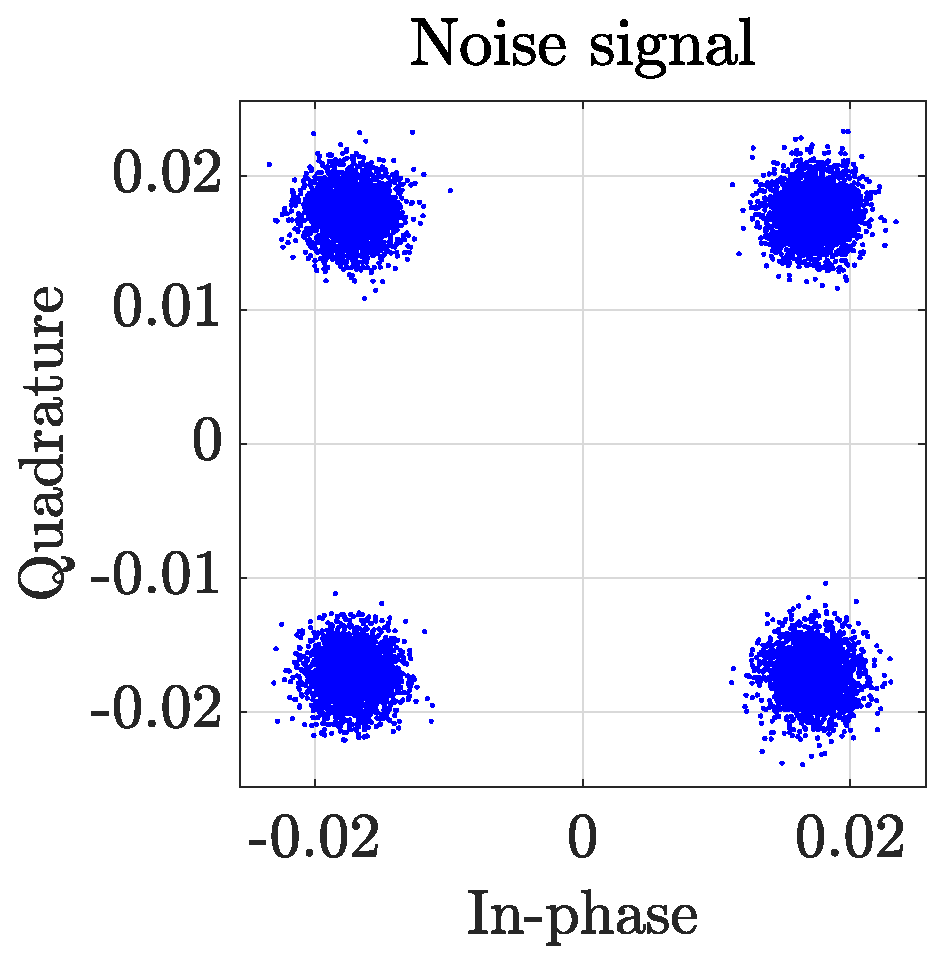
\includegraphics[width=0.5\textwidth]{figures/q01-noised-10000.eps}
    }
    \subfloat[Sinal de saída com rúido]
    {
    \label{fig:output-ac}
	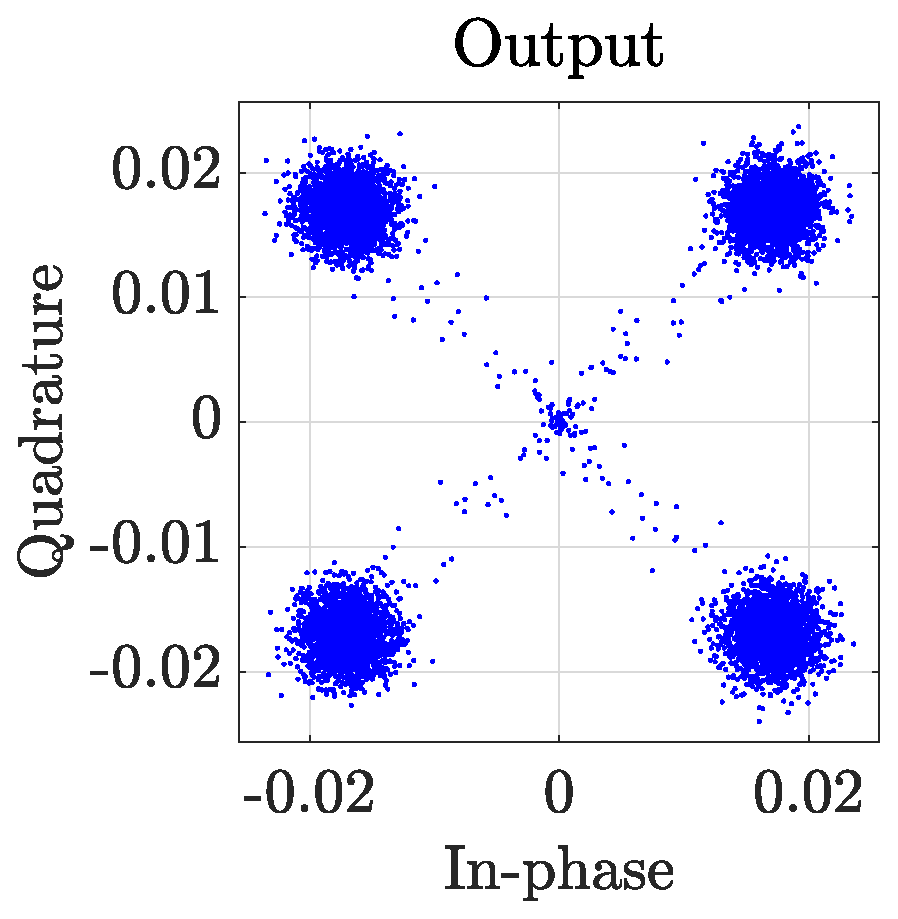
\includegraphics[width=0.5\textwidth]{figures/q01-output-10000.eps}
    }
    \qquad
    \subfloat[Curva de erro]
    {
    \label{fig:Curvas_caract_tensaoCC}
	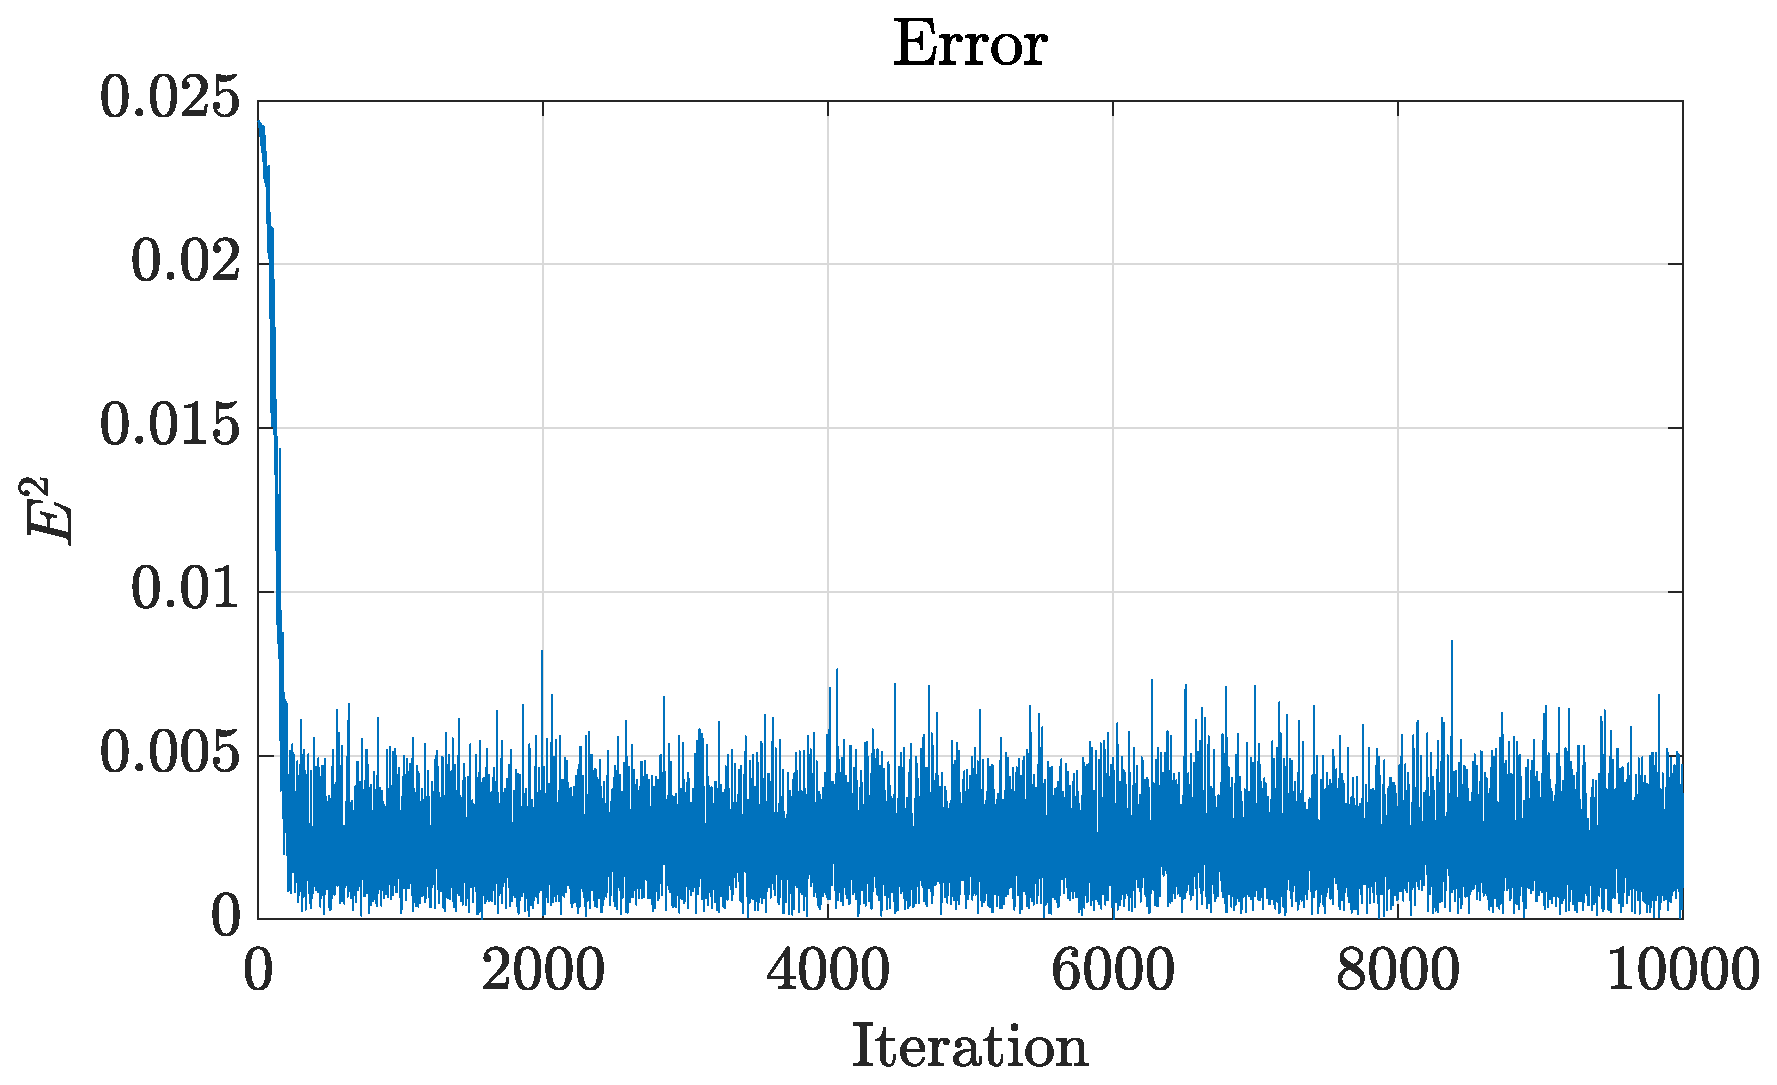
\includegraphics[width=1\textwidth]{figures/q01-error-10000.eps}
    }
	\caption{Resultados das simulação do item (b)}

  \label{fig:input-noise-ab}
\end{figure}

Na Figura \ref{fig:input-noise-c} são exibidos os resultados para um filtro de 20a ordem. Os resultado são similares, quanto à reconstrução do 4-QAM, e quanto à convergência do método em aproximadamente 500 iterações.

\begin{figure}[htb!]
  \centering
  \subfloat[Sinal de entrada com rúido]
    {
    \label{fig:Curvas_caract_tensaoCC}
	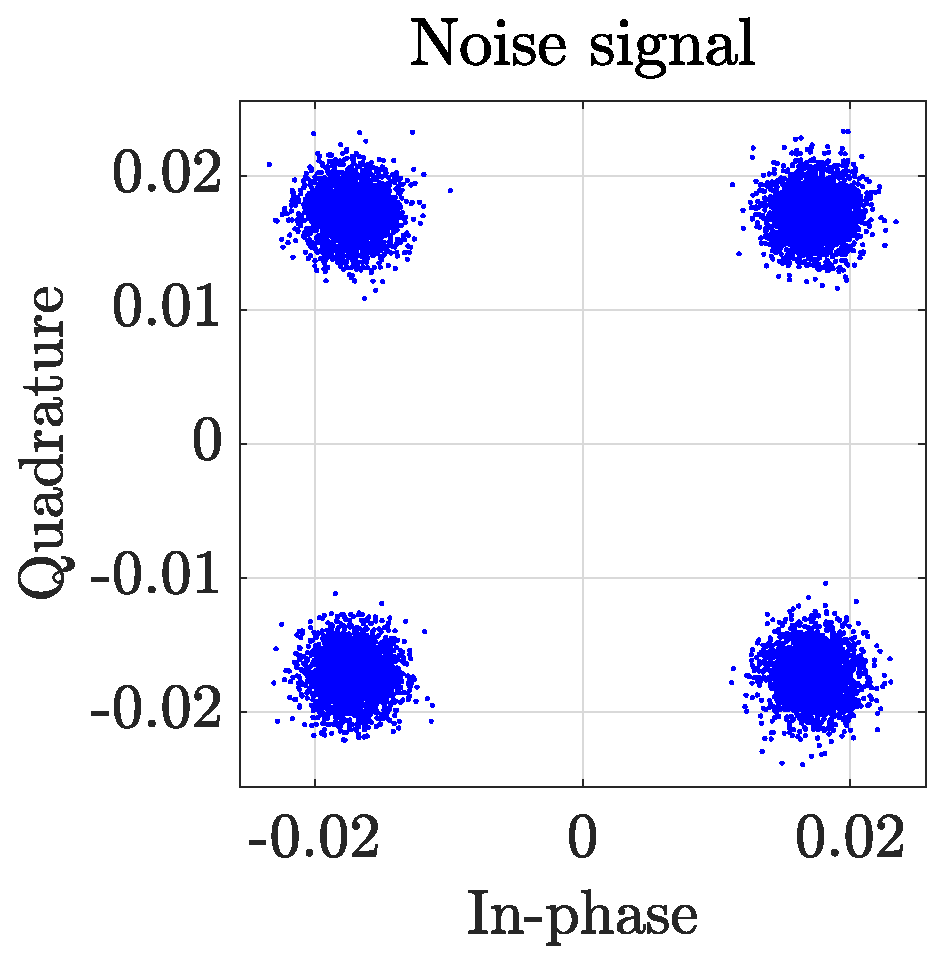
\includegraphics[width=0.5\textwidth]{figures/q01-noised-10000.eps}
    }
    \subfloat[Sinal de saída com rúido]
    {
    \label{fig:Curvas_caract_tensaoCC}
	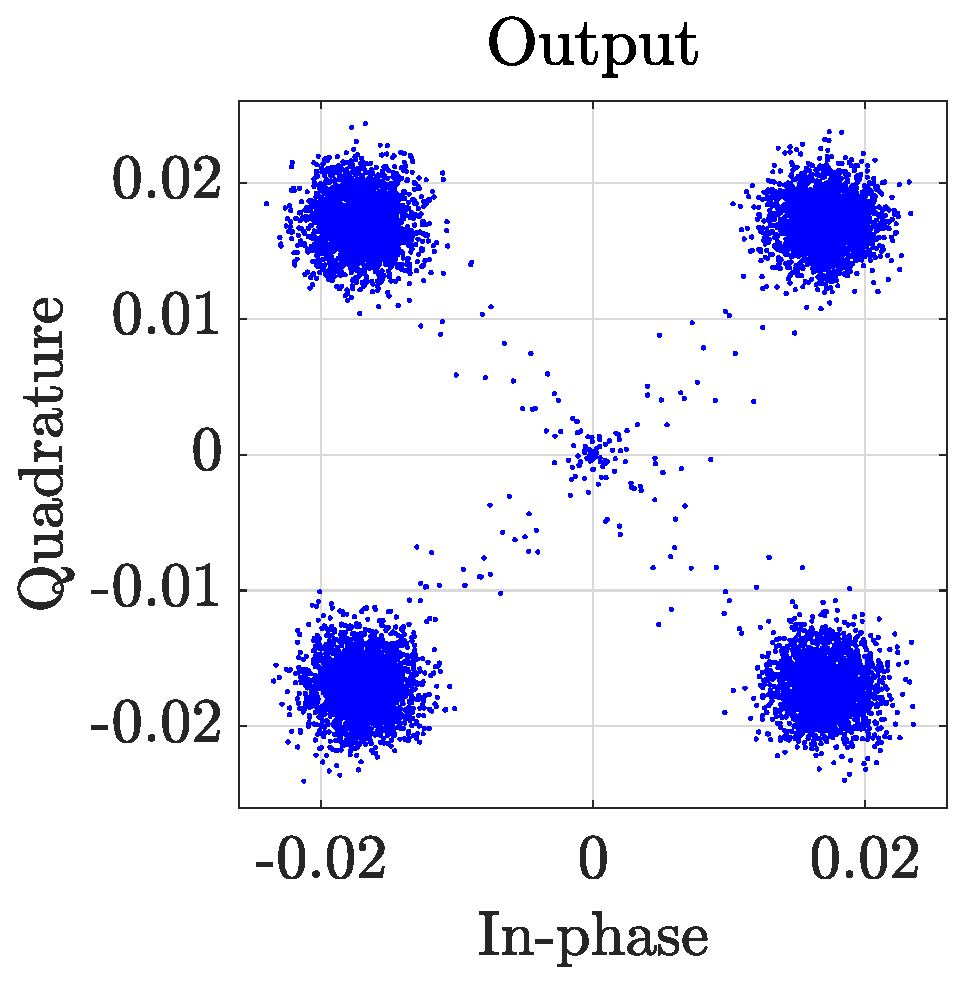
\includegraphics[width=0.5\textwidth]{figures/c-Figures/q01-output-10000.eps}
    }
    \qquad
    \subfloat[Curva de erro]
    {
    \label{fig:Curvas_caract_tensaoCC}
	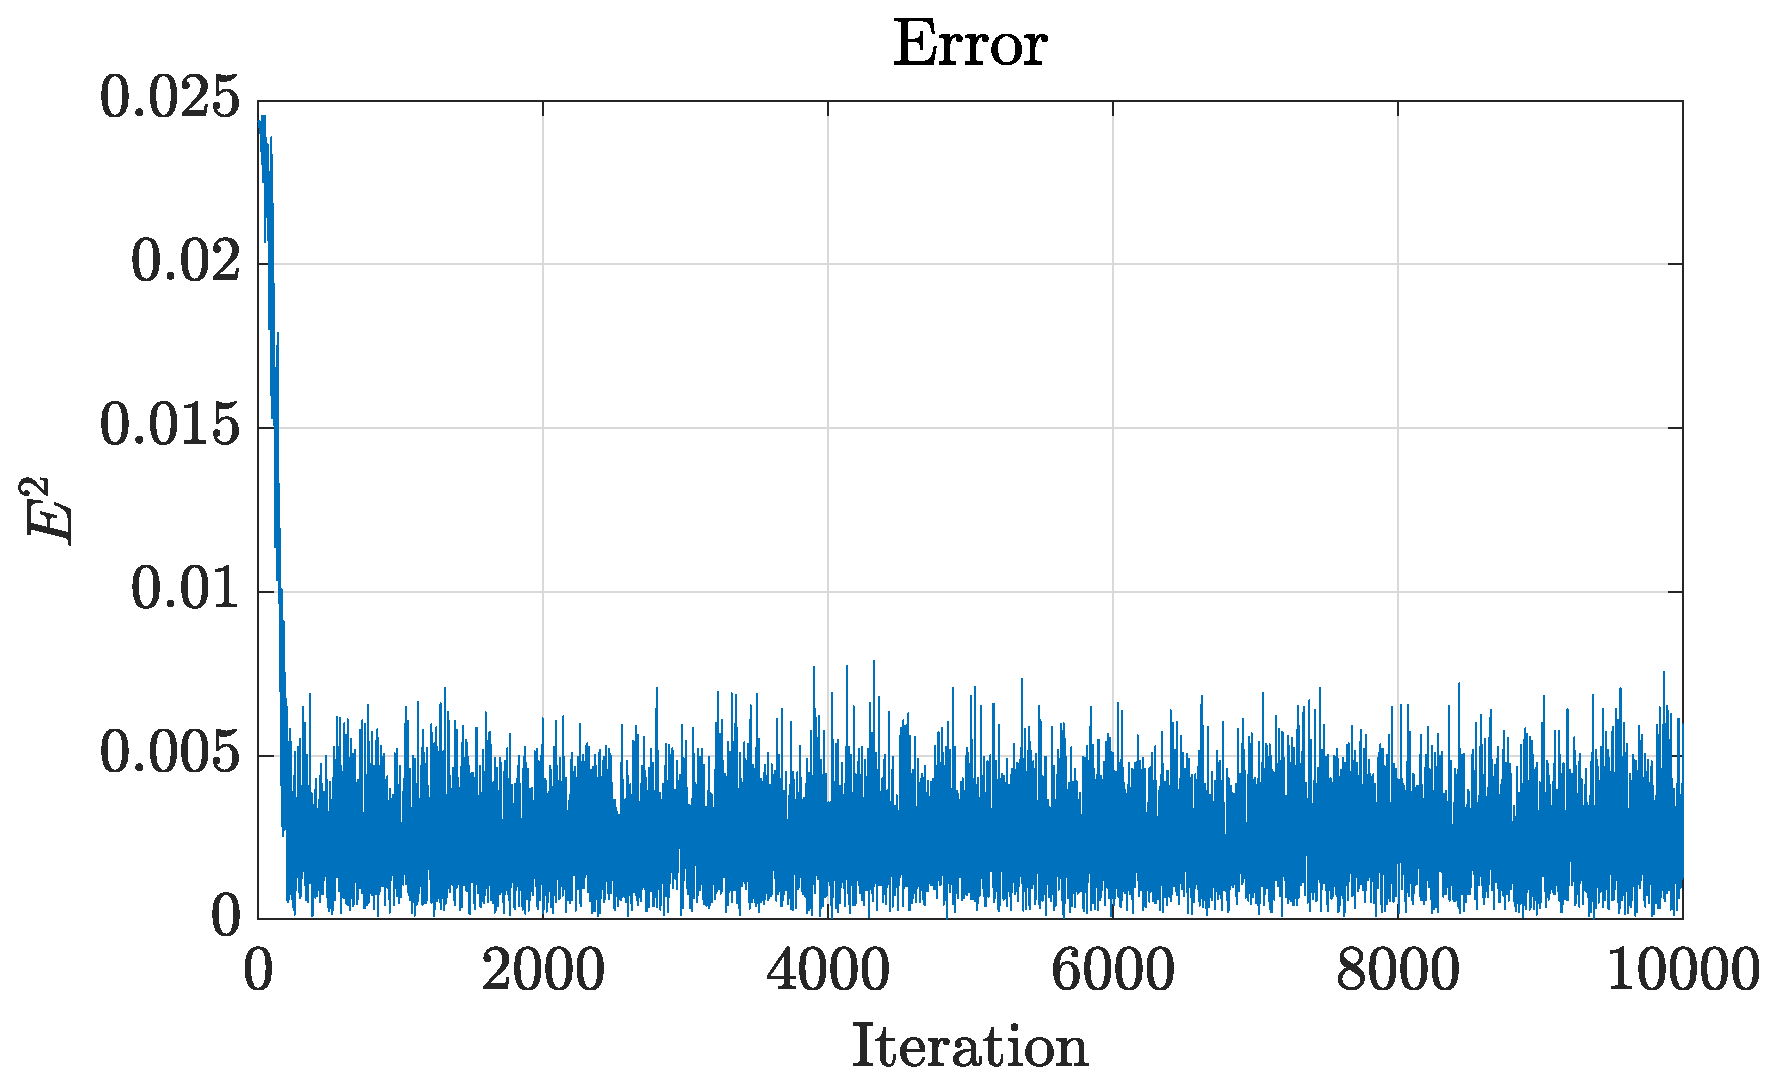
\includegraphics[width=1\textwidth]{figures/c-Figures/q01-error-10000.eps}
    }
	\caption{Resultados das simulação do item (c)}

  \label{fig:input-noise-c}
\end{figure}


\section{Solução}

Os resultados aqui exibidos são baseados em filtragem ITL, específicamente foca em métodos de kernel. Os desenvolvimentos foram baseados no estudos de \cite{vanvaerenbergh2013comparative}.

Foi utilizado o método KRLS, com kernel Gaussiano. A simulações seguiram o mesmo padrão da questão anterior. Entretanto, variou-se a janela do kernel entre 2 e 8 amostras. Os resultados estimados são exibidos na Figura \ref{fig:output-krls}. identificou-se que a reconstrũção do 4-QAM foi melhor obtida do que usando o RLS simples, como na Questão 1, especialmente ao utilizar uma janela de tamanho 2. Percebe-se que com uma janela de tamanho 5 o método começa a não convergir, \emph{i.e.}, não sendo capaz de reconstruir o canal.


\begin{figure}[htb!]
  \centering
    \subfloat[Kernel window = 2]
    {
    \label{fig:Curvas_caract_tensaoCC}
	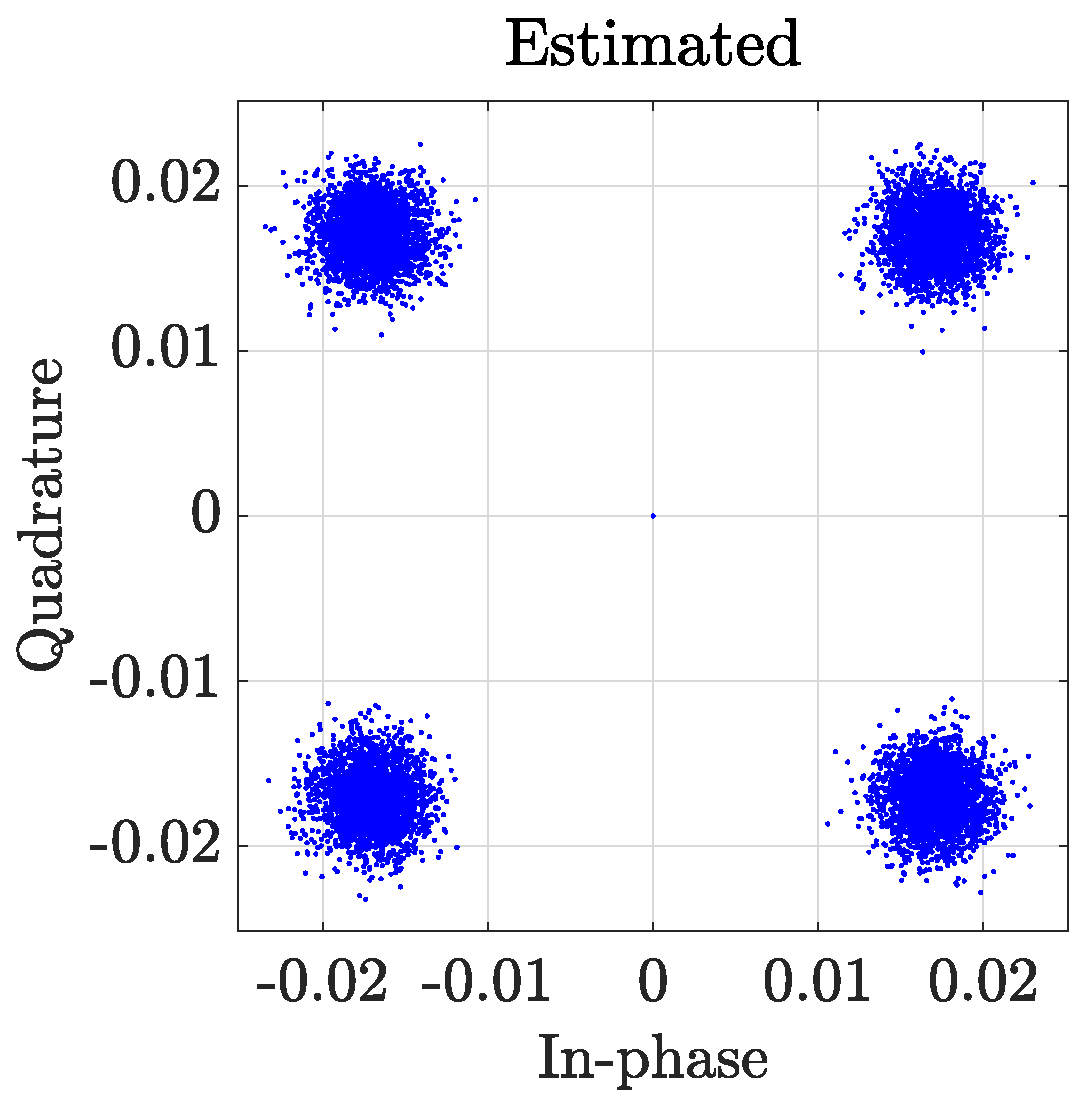
\includegraphics[width=0.5\textwidth]{figures/q2-figures/q02-estimated-10000-gauss-2.eps}
    }
    \subfloat[Kernel window = 4]
    {
    \label{fig:Curvas_caract_tensaoCC}
	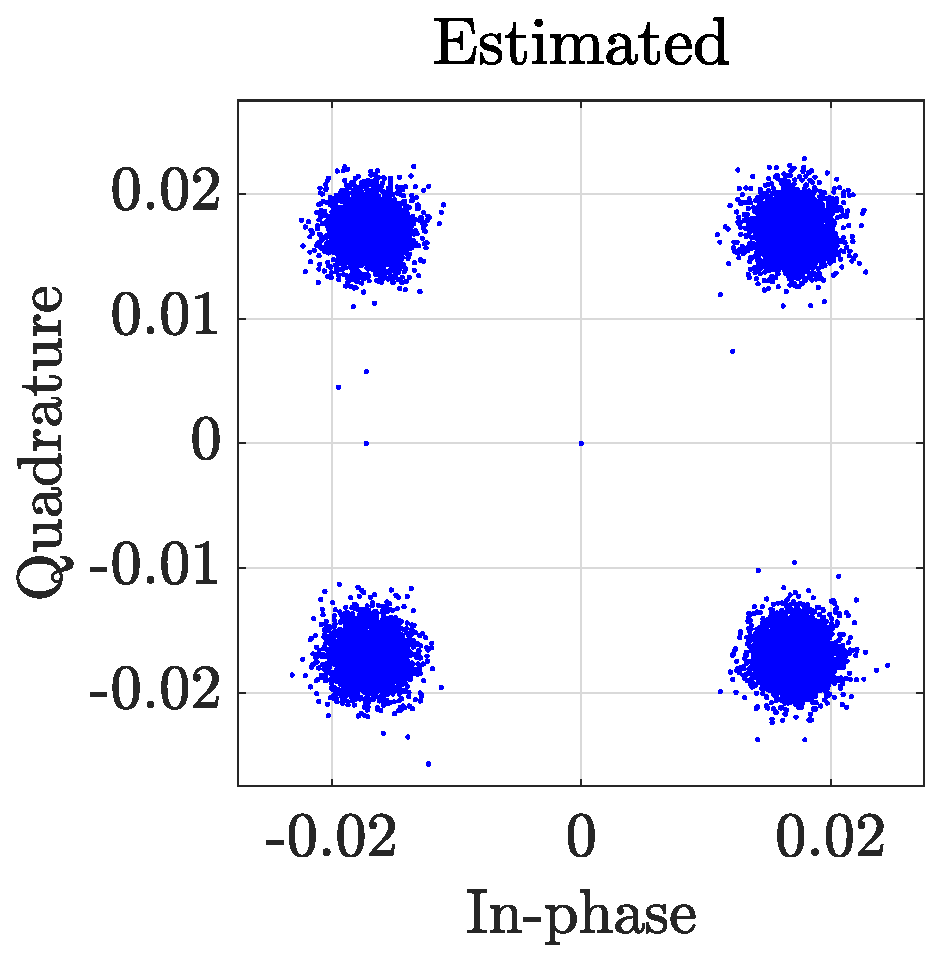
\includegraphics[width=0.5\textwidth]{figures/q2-figures/q02-estimated-10000-gauss-4.eps}
    }
    \\
    \subfloat[Kernel window = 5]
    {
    \label{fig:Curvas_caract_tensaoCC}
	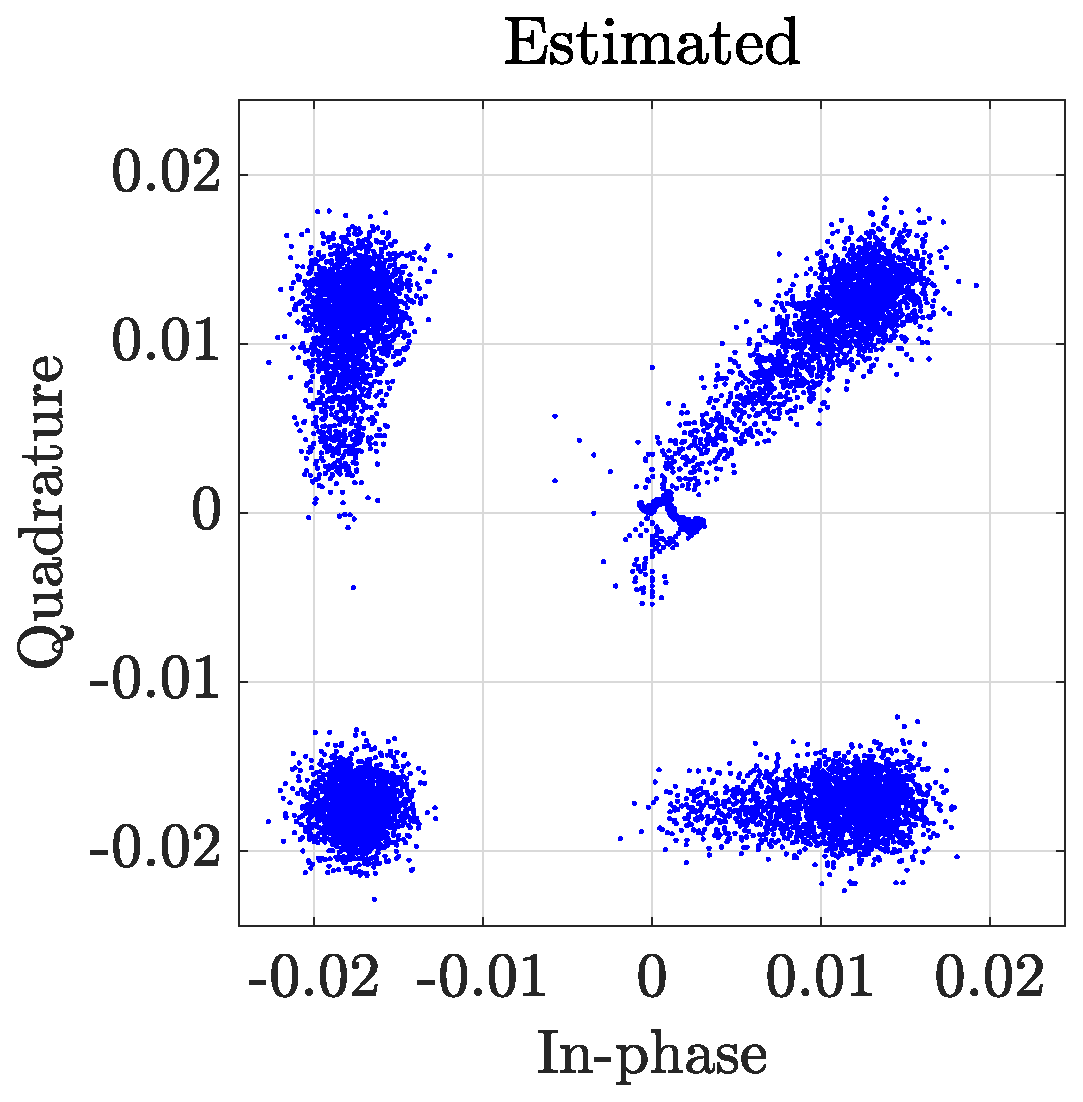
\includegraphics[width=0.5\textwidth]{figures/q2-figures/q02-estimated-10000-gauss-5.eps}
    }
    \subfloat[Kernel window = 6]
    {
    \label{fig:Curvas_caract_tensaoCC}
	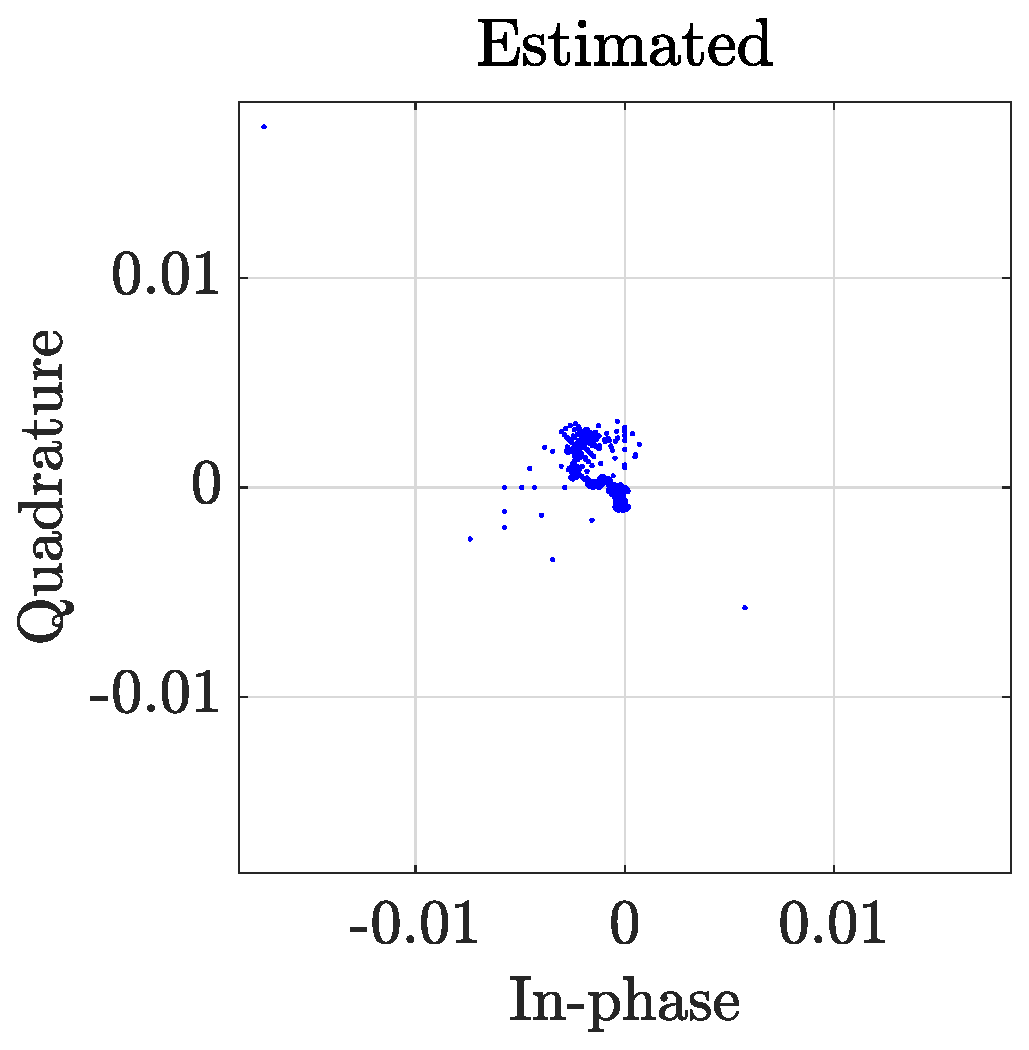
\includegraphics[width=0.5\textwidth]{figures/q2-figures/q02-estimated-10000-gauss-6.eps}
    }
    \\
    \subfloat[Kernel window = 7]
    {
    \label{fig:Curvas_caract_tensaoCC}
	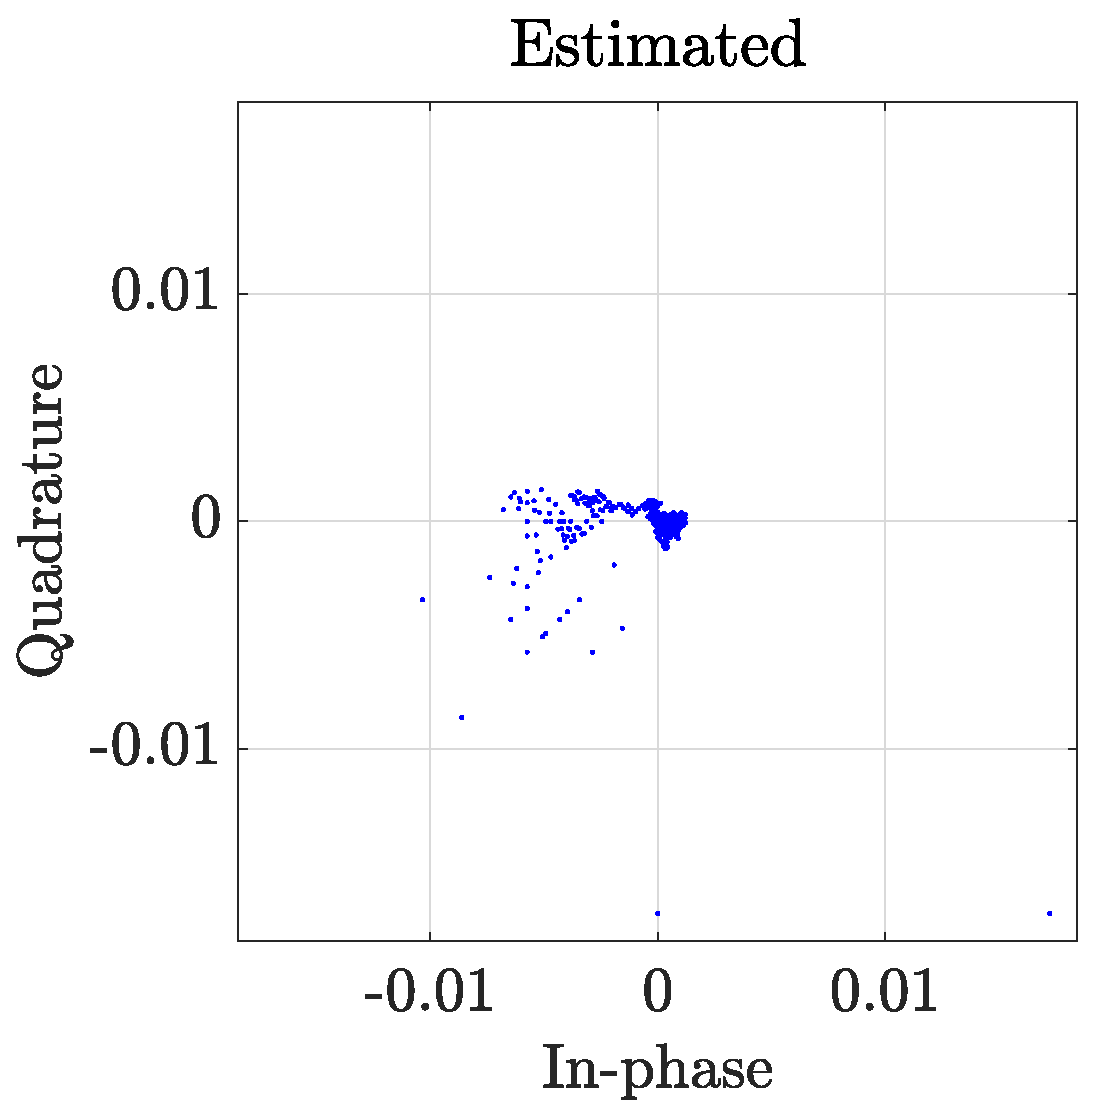
\includegraphics[width=0.5\textwidth]{figures/q2-figures/q02-estimated-10000-gauss-7.eps}
    }
    \subfloat[Kernel window = 8]
    {
    \label{fig:Curvas_caract_tensaoCC}
	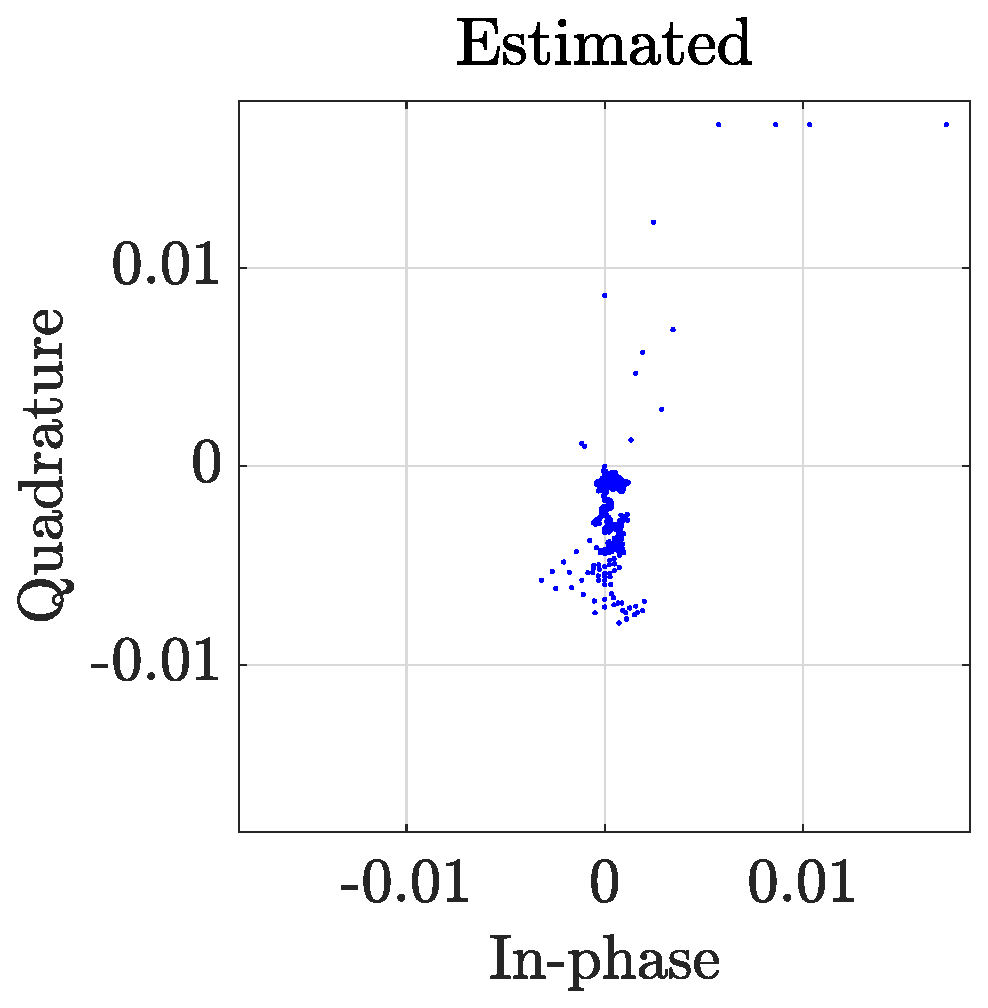
\includegraphics[width=0.5\textwidth]{figures/q2-figures/q02-estimated-10000-gauss-8.eps}
    }
	\caption{Saída estimadas pelo filtro KRLS}

  \label{fig:output-krls}
\end{figure}



% \newpage
\section*{References}

\bibliography{mybibfile}

\end{document}